\chapter{系统总体设计}\label{chap:systemoveral}

在进行系统的设计之前需要了解整个设计的流程,所以本章首先介绍系统设计的框图;除此之外,还将介绍本设计的硬件架构设计方案,并在该小节比较了基于 HLS 设计的硬件加速结构 CNNIOT 相对于 NVDLA 的缺陷;在本文的任务中,还要考虑到资源使用的情况,所以本章还介绍了硬件验证平台的选择;最后,为了方便演示,介绍了本设计的演示页面。

\section{系统设计框图}

本设计的系统的总体设计结构如图~\ref{fig:System Design}所示分为四个阶段:
\begin{enumerate}
    \item 在服务器端,基于 GPU 使用 Caffe 框架训练模型,又因为本设计的硬件加速系统仅支持 INT8 模型的推理,还结合 TensorRT 完成了模型的量化。
    \item 在主机端,使用深度神经网络编译器将已经量化好的模型进行编译与优化,将模型的参数、数据等信息进行序列化压缩,方便传输。
    \item 在 ARM 处理器上,使用深度神经网络运行时将序列化文件进行反序列化,通过 AXI4 总线与硬件加速器 NVDLA 进行通信。
    \item 在 FPGA 上,实现了 NVDLA 的硬件加速器系统,其通过 AXI4 总线协议与外部通信,其内部包含五种引擎(NVDLA 有六个引擎,但因为本设计没有使能第二高速存储,所以 BDMA 引擎并未在本设计中被实现)。
\end{enumerate}

\begin{figure}[!htbp]
    \centering
    \includegraphics[width=0.8\textwidth]{systemDesign.pdf}
    \caption{硬件总体设计架构}
    \label{fig:System Design}
\end{figure}

\section{硬件设计架构与互联}

本设计的硬件总体架构设计如图~\ref{fig:Hardware Design}所示,双核的32位 ARM A9 是本设计的主控制器,通过 AXI4 总线与加速器进行通信。在系统的外部,通过一块 SD Card 来存放 Linux 启动文件与文件系统;通过以太网和外部进行通信;

\begin{figure}[!htbp]
    \centering
    \includegraphics[width=0.6\textwidth]{hardwareDesign.pdf}
    \caption{硬件总体设计架构}
    \label{fig:Hardware Design}
\end{figure}

在设计的初期,加速器(Accelerator,ACC)参考了 CNNIOT\cite{CNNIOT} 设计了通用的卷积神经网络加速器,其支持配置可以调节的卷积、池化、激活函数、全连接等基本卷积神经网络算子。基于该加速器,设计实现了手写数字识别网络 LeNet5,平均处理一张图像需要 168ms,而 Arm A9 处理一张图像需要 1204ms。为了实现整个网络,需要:

\begin{enumerate}
    \item 使用 Caffe 预训练模型得到 Caffemodel 文件。
    \item 使用 Netron 将 Caffemodel 文件内部的权重参数导出为二进制文件。
    \item 由加速器设计神经网络结构,并进行推理。
\end{enumerate}

针对仅有三层卷积层,两层全连接层的 Lenet5 网络来说,配置的过程已经十分复杂,更不用说设计包含残差结构的 Resnet 网络。由此可以看出,硬件加速器被设计出来只是第一步,还需要构建完整的软件栈体系。

在经过一番调研之后,加速器设计选择了英伟达公司开源的 NVDLA 框架,经过英伟达团队几年的努力,NVDLA 自上而下打通了软件栈与硬件栈,可以实现端到端的推理,是一个适合深入学习的框架。

在 Xilinx 的设计工具中提供的 IP 核大多使用 AXI4 总线来实现各级之间的逻辑控制和数据传输。前文中提到,NVDLA 亦是使用 AXI4 总线访问存储,无疑极大方便了我们的设计,但是 NVDLA 的控制总线协议不是 AXI4 协议,在本设计中,其通过 csb2apb 电路将 CSB 协议转换为 APB 总线协议,在 Vivado 设计中,我们使用 Xilinx 官方提供给的 APB2AXI Bridge IP 将 APB 总线再转换为 AXI4 总线挂载到 ARM 处理器上。

\section{验证平台}

NVDLA 的驱动程序需要挂载到 Linux 内核上,所以本设计需要一款通用处理器作为主控,并且为其移植 Linux 操作系统。并且,考虑到本设计采用的 small 配置需要7万以上的查找表资源。则可供选型的器件型号有:

\begin{enumerate}
    \item ZYNQ 7000 系列,该芯片集成了一块双核32位 ARM A9 处理器作为主控制器,而 FPGA 侧的资源随芯片的型号不同而不同,想要实现 NVDLA 至少需要使用到 ZYNQ 7045 器件。
    \item ZYNQ MPSoc 系列,该芯片集成了一块多核的64位的 ARM A53 处理器作为主控制器,性能相较于 ZYNQ 7000 器件强,官方开发板卡的价格在2万左右。
    \item 纯 FPGA 逻辑器件,如官方板卡 VCU118,有足够大的LUT资源,可以将 RISC-V 处理器与 NVDLA 一起实现,并在 RISC-V 处理器上移植 riscv-linux,开发周期较长。
\end{enumerate}

综合以上,本设计选用的器件型号为 XC7Z045-2FFG900I,开发板卡为如图~\ref{fig:ZYNQ 7045}的第三方板卡,价格为三千多元人民币。

\begin{figure}[!htbp]
    \centering
    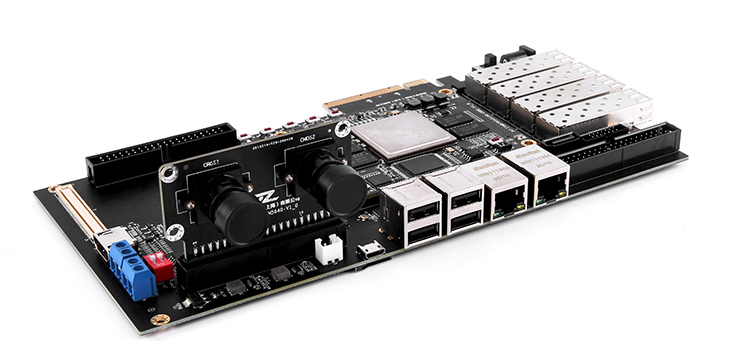
\includegraphics[width=0.8\textwidth]{ZYNQ 7045.jpeg}
    \caption{ZYNQ 7045 开发板}
    \label{fig:ZYNQ 7045}
\end{figure}

\section{用户友好的输入页面设计方案}

如图~\ref{fig:BootStrap}所示,本设计基于 Bootstrap 与 Flask 等 Web 应用技术开发了用户友好的输入页面与数据显示页面。

\begin{figure}[!htbp]
    \centering
    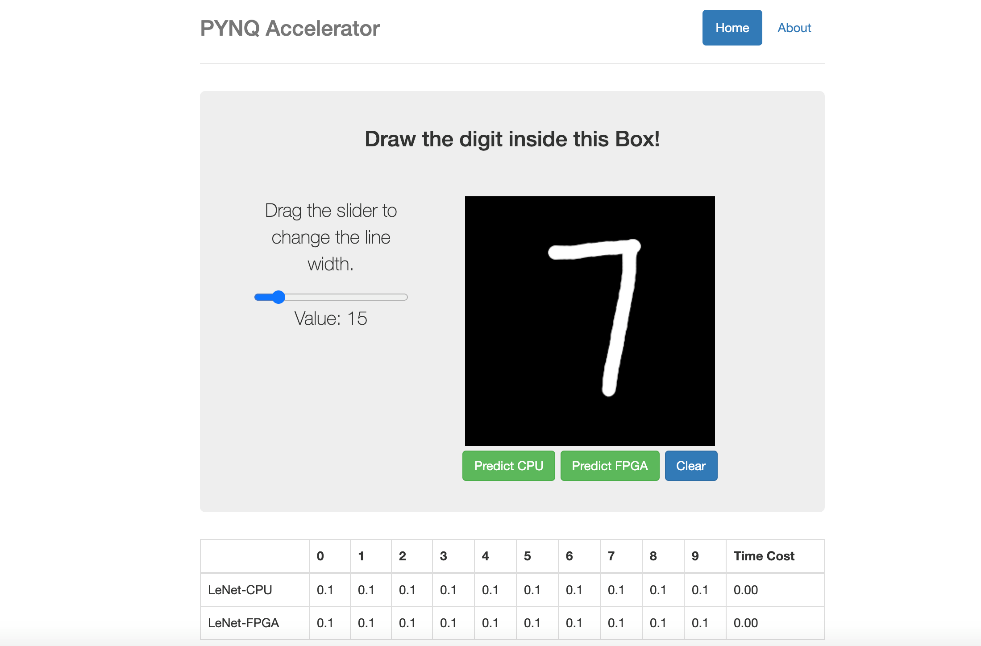
\includegraphics[width=0.7\textwidth]{bootstrap}
    \caption{用户友好的输入页面}
    \label{fig:BootStrap}
\end{figure}

Bootstrap 是由 Twitter 推出的用于前端开发的开源工具包,它简洁灵活,功能强大,本次设计初始阶段使用 Bootstrap 设计了一个手写数字页面,用户可以通过鼠标在 Canvas 画布上调节画笔大小,绘制数字,通过按键来决定采用 ARM 或者 FPGA 进行深度神经网络的推理。

当用户按下按键之后,Web 前端会使用 Ajax 发送 HTTP 请求,通过以太网与开发板通信,获取处理结果。在板卡上,本设计使用 Flask 部署了Web应用的后端,负责接受 HTTP 请求,决策推理平台,将推理结果以及相关信息打包发送 HTTP 响应。
